\chapter{Elements of fracture mechanics and DIC method}
\label{Chapter2}

\section{Pre and Post processing work preparation}

\subsection{MMCG test piece}

The MMCG test piece was developed by Moutou Piti [MOU 2008]. However, the specimens tested at the University of Lisbon are not of the same dimensions. After carefully measuring the specimens, it turns out that they have the same dimensions as the specimens studied by Odounga. Below are the dimensions of the specimens that will be tested figure \ref{fig:fig23}:

\graphicspath{{Images/}}
\begin{figure}[htp]
	\centering
	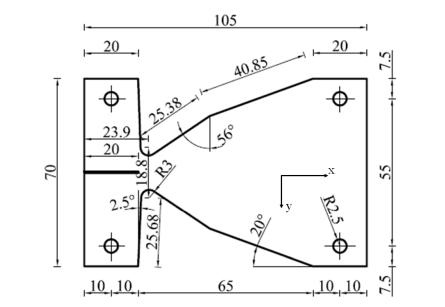
\includegraphics[width=8cm]{fig23}
	\caption{Dimensions of the tested MMCG specimen}
	\label{fig:fig23}
\end{figure}

\subsection{Arcan model and final grips}

To perform the tests, a steel Arcan system must be designed. It is made of high tensile steel (HLE). Indeed, this part allows to connect the 2MCG wood specimen to the press. In order to create this grip we must first take into account the dimensions of the 2MCG specimen available in Nova school described in figure \ref{fig:fig24}. The shape of the Arcan system must also allow a good visibility on the propagation of the crack. Figure 21 shows the Arcan device that we will use, which was inspired from the thesis of [ODO 2018].

\graphicspath{{Images/}}
\begin{figure}[htp]
	\centering
	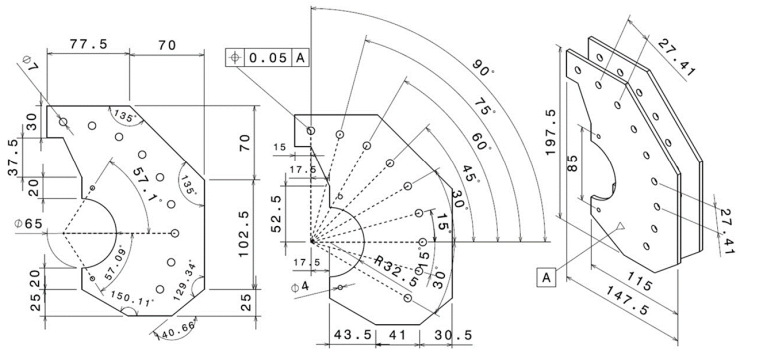
\includegraphics[width=10cm]{fig24}
	\caption{Size of the Arcan fastening system[ODO 2018]}
	\label{fig:fig24}
\end{figure}

The fixing holes for the wooden specimens have a diameter $\Phi= 5 mm$, and the loading holes have a diameter $\Phi = 7 mm$. These fixing holes were drilled in order to be able to load the specimen with different angular values of the angle in relation to the vertical direction in order to activate different failure modes depending on the load angle. To connect the Arcan system to the press, a piece had to be created, as shown in figure \ref{fig:fig25}.

\graphicspath{{Images/}}
\begin{figure}[htp]
	\centering
	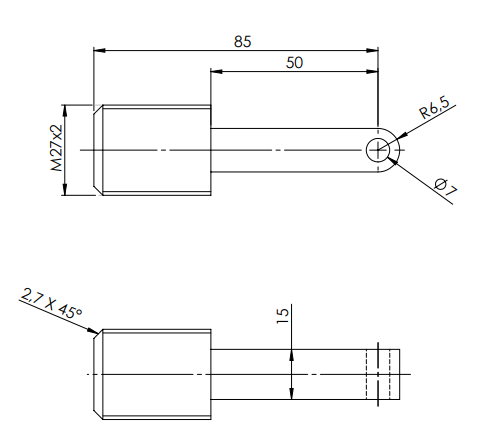
\includegraphics[width=6cm]{fig25}
	\caption{Bolt for connecting the press and the Arcan System}
	\label{fig:fig25}
\end{figure}

This part has a hole of the same size as the holes of the Arcan system in order to connect them. Moreover the head of the connector is 27mm in diameter and the thread has a 2mm pitch to connect to the press. Before sending the technical drawings to a company, a 3D printer was used to verify that the system worked properly. It was then necessary to draw the assembly on solidworks in order to print the assembly and send the technical drawings. Figure \ref{fig:fig26} shows the assembled device in Solidworks.

\graphicspath{{Images/}}
\begin{figure}[htp]
	\centering
	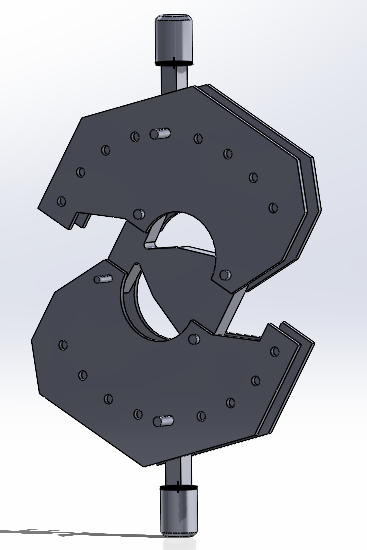
\includegraphics[width=5cm]{fig26}
	\caption{Assembled device in Solidworks}
	\label{fig:fig26}
\end{figure}

It has been shown in previous work such as [ODO 2018] that one of the main problems with the MMCG specimen is the small distance between the holes and specimen extremities. This implies several cracks in the heel between the hole and the extremity of the sample which prevents observation and analysis of the fracture. One solution proposed by Odounga is the use of washers. Indeed, by applying compressive stress on each side of the sample, it reduces the stress applied on the holes and distributes the load in a wider area.

\subsection{Hydraulic press used}

To determine experimental parameters like the load speed or the frequency of the camera recording, it was important to read previous works on the subject and determine which engines will be used to proceed the experiments. The press used for the tests is a Landmark Servohydraulic Test Systems model 661.21B-03  from MTS. It is capable of exerting a maximal applied load of 10 metric to N (figure \ref{fig:fig27}).
In the work of Ostapska and Malo [KAT 2021] the load speed recommended was about $0.1\ mm\ {min}^{-1}$ and the record was made at a frequency of 5 Hz, so 5 images per seconds. In the work of Mambili the record was made at a frequency of 10 Hz and the load speed was about 0.3 mm/s with a pre-load of 100N. It should be remembered that this press is also chosen because of its ability to load the specimens with a constant time displacement. Indeed, it was explained that this work will use the complacency method to compare the results.

As explained Stanislas Malfait [MAL 2021]  this MTS Hydraulic Press works with a cooler fluid. Indeed, a tank full of fluid mixed to water and a cooler system send this fluid mix to the press as visible on 23. Then, a hydraulic supply from MTS sends this liquid to the press itself. It is the model 506.02 serie 22 coupled with the Vickers DG4V-3-2A. Then the pressure is created thanks to the Hydraulic Service Manifold part from MTS company, model 234.11. Finally, a servo valve MOOG A076-263c increase the pressure to allow the hydraulic press operation. It is a high performance valve which drives a dry torque motor. Then a MTS load cell (661-21B-03) allows to follow the displacement of the hydraulic press.

\graphicspath{{Images/}}
\begin{figure}[htp]
	\centering
	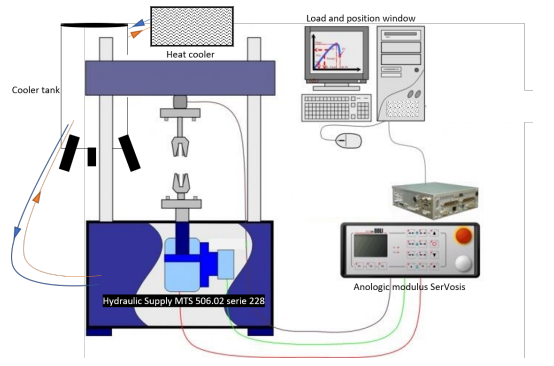
\includegraphics[width=10cm]{fig27}
	\caption{Hydraulic Press components allowing it use[MAL 2021]}
	\label{fig:fig27}
\end{figure}

\subsection{Specimen preparation}

\subsection{Notch and precrack}

Notches were created in each specimen. A precrack is made by a cutter into the notch. The interest is to initiate a straight crack, thanks to this first one. The notch width is around 1.5mm, done by a straight electrical saw. The cutter allow to go deeper and create a precrack with a shape allowing the propagation of the crack. The precrack must be done at the center of the sample heel. Indeed, even a little eccentricity could cause a deviation of the crack and prevent a good study of the propagation. The specimen was designed with an initial crack noted $a_i$ of length  $a_i=22mm$. The total crack length is equal to: $a=a_i+\Delta a$.